\documentclass[a0,portrait]{a0poster}

\usepackage{multicol}
\columnsep=100pt
\columnseprule=3pt
\usepackage[svgnames]{xcolor}
\usepackage{palatino}
\usepackage{amsmath}
\usepackage{graphicx}
\usepackage{booktabs}
\usepackage[font=small,labelfont=bf]{caption}
\usepackage{amsfonts, amsmath, amsthm, amssymb}
\usepackage{wrapfig}
\usepackage{caption}
\usepackage[caption=false]{subfig}
\usepackage{textcomp}
\usepackage{bm}
\usepackage[superscript,biblabel]{cite}
\usepackage{pifont}
\usepackage{xcolor}
\definecolor{myblue}{RGB}{110,0,119}

\newcommand{\bi}{\item[\color{myblue}\ding{108}]} 

\begin{document}

\begin{minipage}[b]{0.80\linewidth}
\veryHuge\centering\color{myblue} 
\textbf{Nonadiabatic simulations of carbon monoxide photodissociation in H64Q neuroglobin} 
\color{Black}\\[1cm]
\huge \textbf{\underline{J. Rydzewski} and W. Nowak}\\
\Large\textit{Institute of Physics, Faculty of Physics, Astronomy and Informatics, Nicolaus Copernicus University, Grudziadzka 5, 87-100 Torun, Poland}
\end{minipage}
%
\begin{minipage}[b]{0.20\linewidth}
\centering

\includegraphics[width=11cm]{umk.png}
\end{minipage}

\vspace{1cm}

\begin{multicols}{2}

\section*{\centering\color{myblue} INTRODUCTION}

\begin{itemize}
\setlength\itemsep{0.6cm}
\bf
	\bi Carbon monoxide (CO) is a leading cause of poisoning deaths worldwide, without available antidotal therapy;
	\bi The potential antidotal treatment paradigm for CO poisoning as introduced by Azarov et al.\cite{0}, is based on near-irreversible binding of CO to H64Q neuroglobin (Ngb) in which the distal histidine six-coordinating the heme iron was mutated to glutamine;
	\bi There is still little known about the exact atomistic mechanism of CO hijacking by H64Q Ngb, which hampers a rational development of similar therapeutic proteins. Therefore, an investigation of interprotein CO migration clusters and geminate recombination of CO within H64Q Ngb is important to fully comprehend CO scavenging;
	\bi Ligand diffusion is not trivial to model computationally, yet it is very important when atomistically-detailed ligand diffusion pathways are virtually not available experimentally\cite{1,2,3,4};
	\bi We focus on the binding of CO to wild type (WT) Ngb and the mutant H64Q, addressing an atomistically-detailed structural mechanism responsible for the recently introduced ligand-trap antidote for CO poisoning and its kinetic determinants.
	
\end{itemize}

\section*{\centering\color{myblue} METHODS}

We employed a methodology comprising (a) unbiased MD simulations of the six-coordinate WT Ngb and H64Q Ngb liganded by CO and (b) nonadiabatic Landau-Zener MD that enables transitions of the system between the ground and the excited states of WT Ngb and H64Q Ngb.

\vspace{1cm}

\begin{center}
	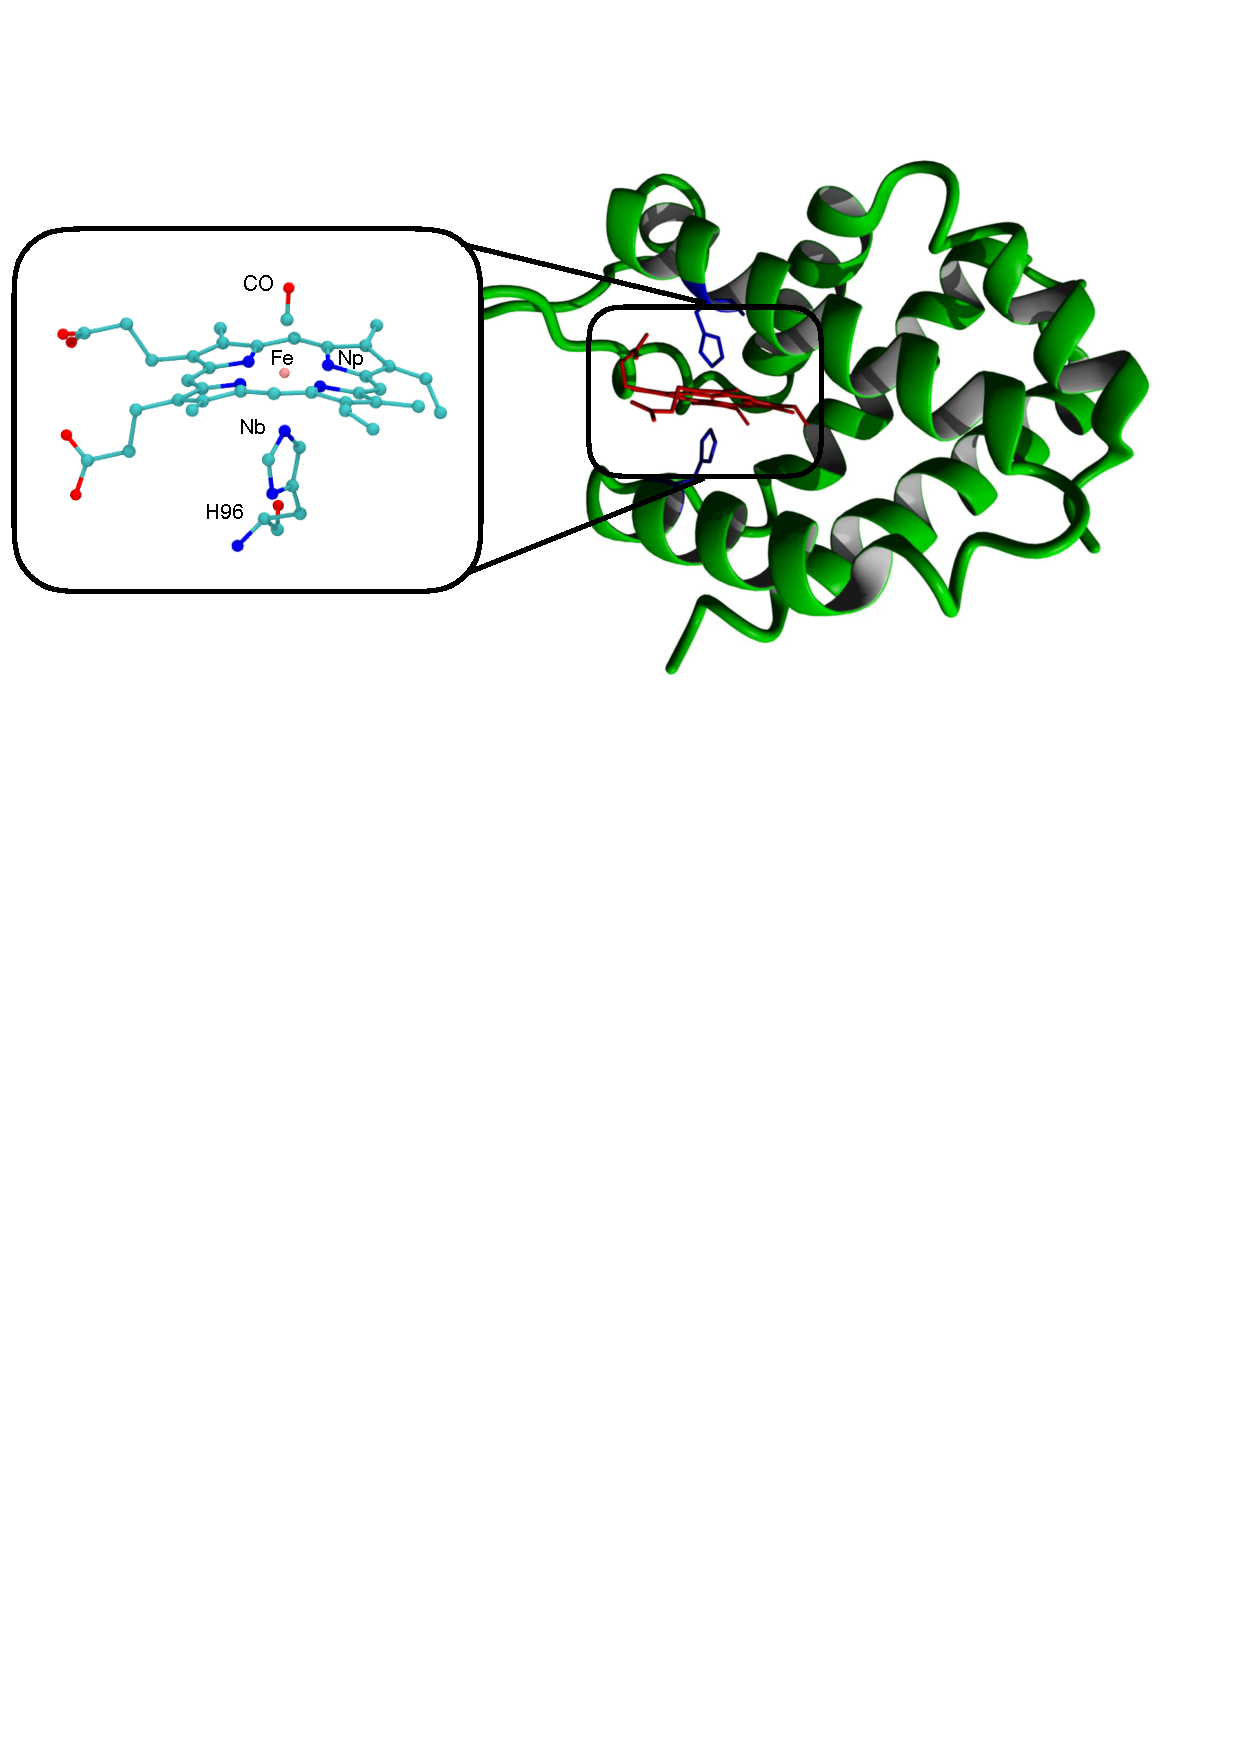
\includegraphics[clip,width=1\columnwidth]{watoc.pdf}%
	\end{center}
	\captionof{figure}{Six-coordinate liganded heme with the proximal histidine (H96) and CO bound. The heme pyrrole nitrogen atoms are shown as Np in blue and the proximal histidine nitrogen atom is shown as Nb in blue.}

\vspace{1cm}

\begin{center}
	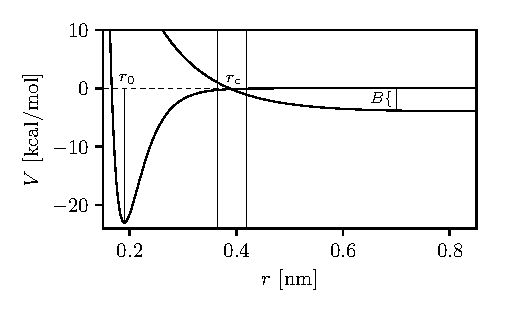
\includegraphics[clip,width=0.48\columnwidth]{figs2.pdf}%
	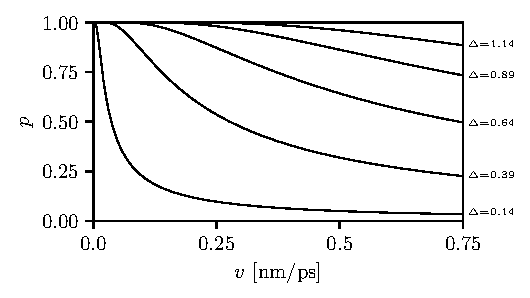
\includegraphics[clip,width=0.52\columnwidth]{figs3.pdf}%
\end{center}
\captionof{figure}{(a) The diabatic energy curves used in the LZ model in the nonadiabatic simulations. (b) The LZ hopping probability for different values of the electronic coupling (in kcal/mol).}

\vspace{1cm}

The diabatic energy curves were modeled by the following equations:  

\begin{equation}
	V_1(r)=D\left[\operatorname{e}^{-2\alpha(r-r_0)}-2\operatorname{e}^{-\alpha(r-r_0)}\right]
\end{equation}

and

\begin{equation}
	V_2(r)=A\operatorname{e}^{-br}-B,
\end{equation}

where $D$ is the binding energy of CO to heme in Ngb, $\alpha$ is the width of the well, $r$  is the reaction coordinate (e.g., the distance between the heme iron and the carbon atom of CO), $r_0$ is the equilibrium length of the Fe-CO bond, $A$ and $b$ are parameters, and $B$ is the difference between the diabatic energy curved when the system is dissociated. The parameter describing the conical intersection is denoted by $r_c$.

The transitions between electronic diabatic curves are modeled in our approach in two ways. 
\begin{itemize}
	\bi A direct absorption of a photon that takes the system from the ground to the excited state without any change in the nuclear positions and velocities. The absorption is restricted by the Franck-Condon overlap. At any point in a simulation, a photon can be absorbed with a constant probability of 0.1 photon/ps.

	\bi The Landau-Zener model\cite{lz}. We consider the probability $p$ of the system to remain on a diabatic energy curve while passing through the conical intersection. The probability is given by $p=\exp(-\pi\sigma)$ and $\sigma=\pi\Delta^2/hvf$, where $\Delta$ is the electronic coupling between the diabatic curves, $h$ the Planck constant, $v$ the modulus of velocity of the reaction coordinate (i.e., the distance between the Fe from the heme moiety and the carbon of CO), and $f$ the difference of the special derivatives of the diabatic curves at the conical intersection.
\end{itemize}

\section*{\centering\color{myblue} RESULTS}

\vspace{1cm}

\begin{center}
	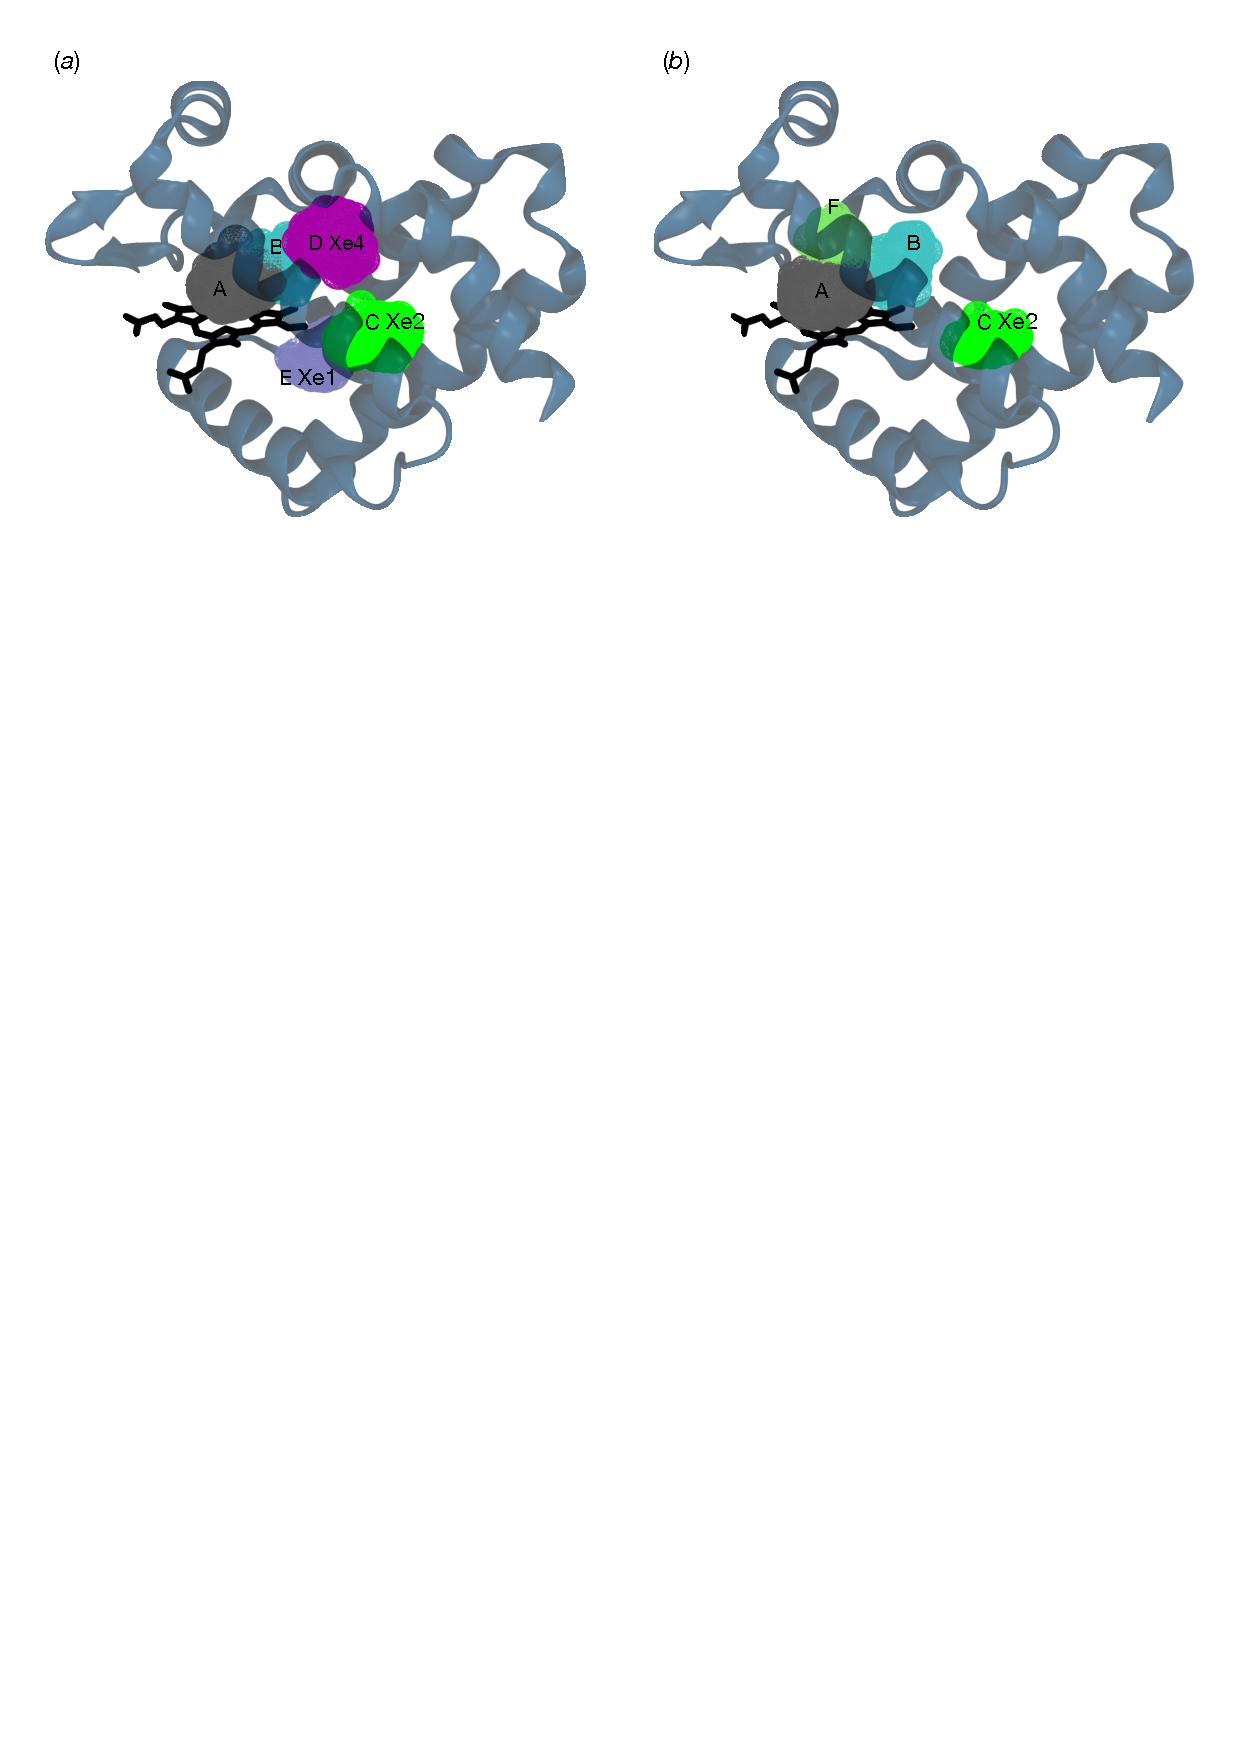
\includegraphics[clip,width=\columnwidth]{fig1.pdf}%
\end{center}
\captionof{figure}{Clusters of CO within the system comprising Ngb (transparent blue) and the heme moiety (black licorice). The calculated clusters are labeled by letters. (a) CO migration clusters in WT Ngb and their population: A (56\%), B (14\%), C Xe2 (7\%), D Xe4 (6\%), E Xe1 (1\%) and CO conformations clustered as noise, which consisted mainly of the photodissociated CO outside Ngb (16\%, not shown). (b) CO migration clusters in H64Q Ngb and their population: A (74\%), B (4\%), C Xe2 (1\%), F (1\%) and noise (20\%, not shown).}

\vspace{1cm}

\begin{center}
	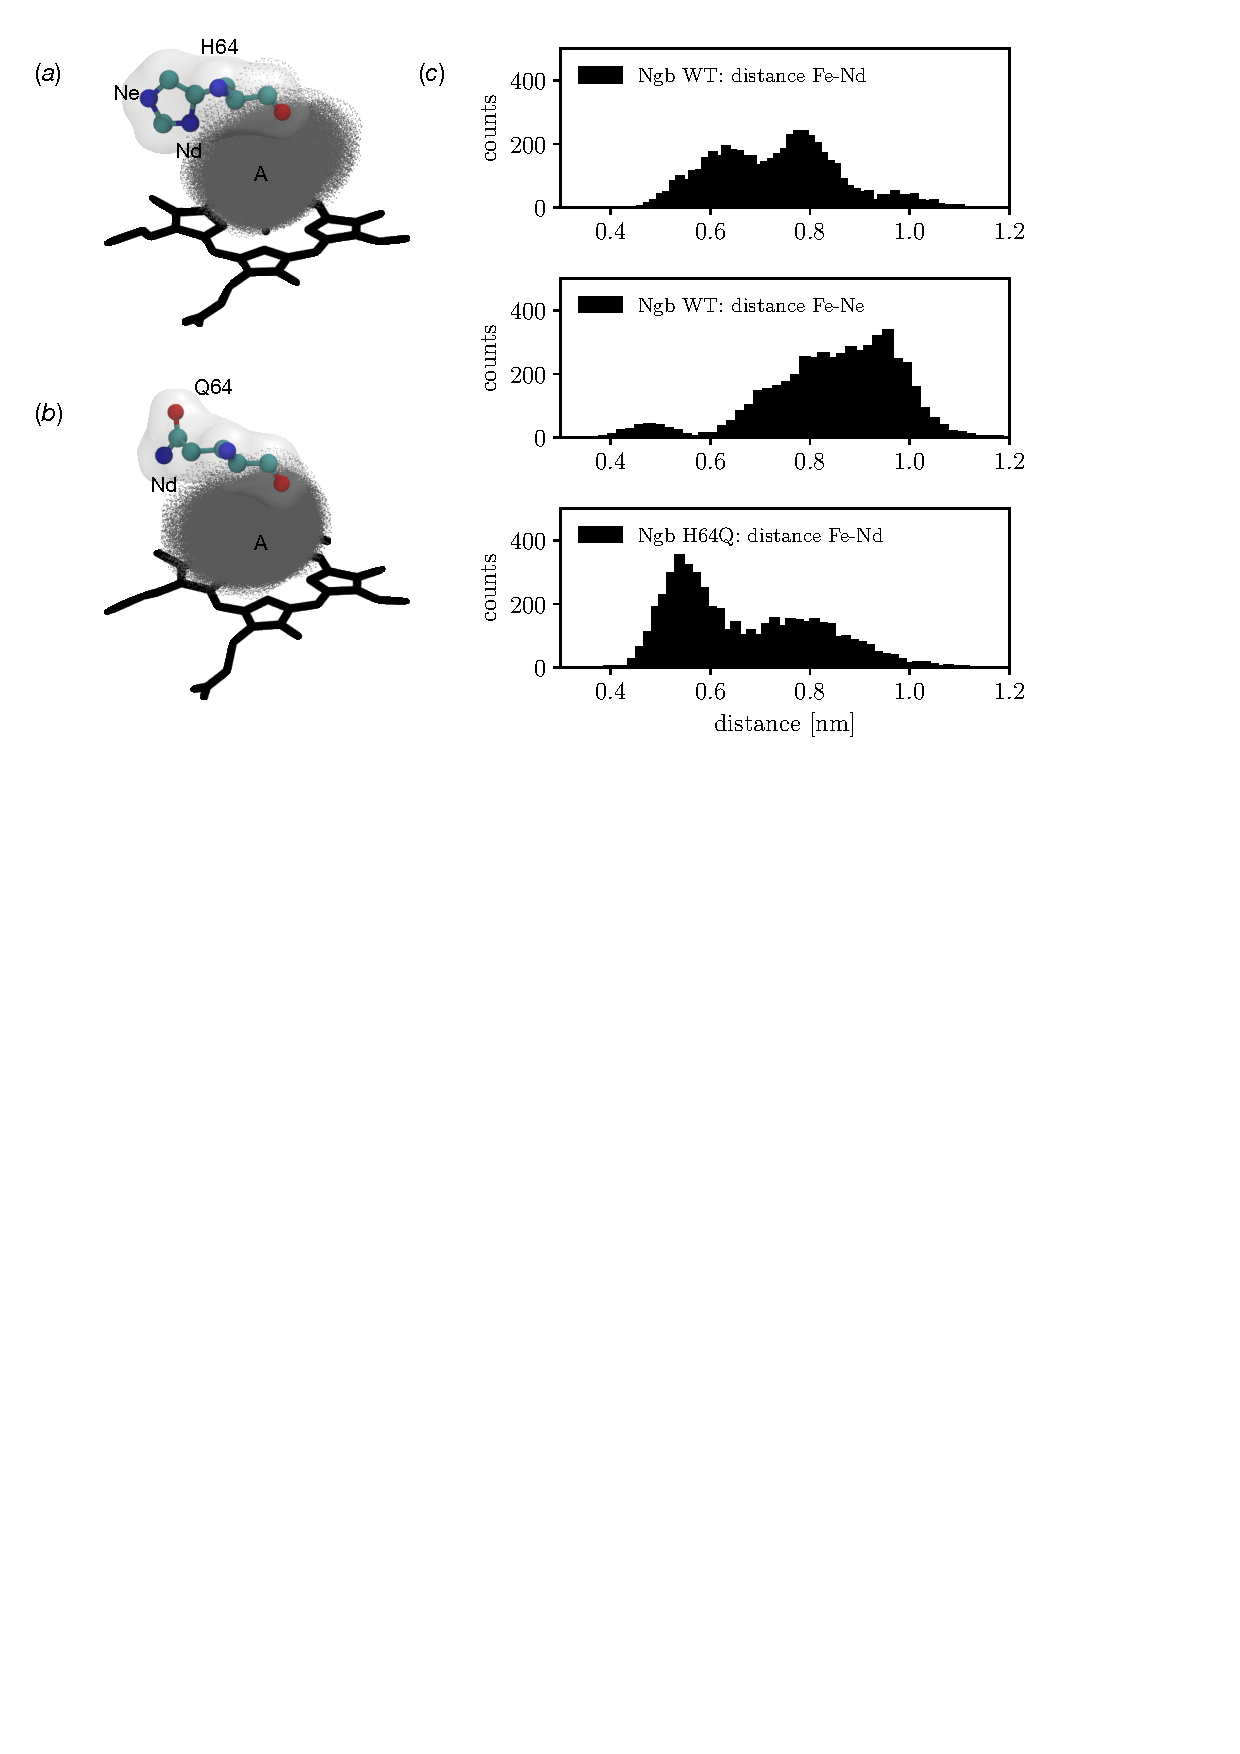
\includegraphics[clip,width=\columnwidth]{fig2.pdf}%
\end{center}
\captionof{figure}{CO distribution in the distal heme pocket with the amino acids responsible for the shape of the cluster A–(a) H64 for Ngb WT and (b) Q64 for Ngb H64Q shown as licorice. (c) Histograms of distance between the labeled nitrogen atoms (Nd and Ne from Ngb WT and Nd from Ngb H64Q) and the heme iron.}

\section*{\centering\color{myblue} CONCLUSIONS}

\begin{itemize}
\setlength\itemsep{1cm}
	\bi Our study shows the differences in the CO distributions in the Ngb matrices of the wild type and mutant, depicting the hijacking behavior of the cluster A, that limits the CO migration to the rest of the determined clusters;
	\bi This finding agrees with the observation showing that H64Q Ngb engages in the CO geminate recombination 2.7 times more frequently than WT Ngb, which indicates that the distal histidine substitution by glutamine results in weakened competition with CO for the optimal length of the Fe-CO bond along the normal to the heme plane;
	\bi We presented a general approach that can be used in other photoactive systems comprising thousands of atoms instead of quantum dynamics. This study may provide the molecular basis for the rational design of next-generation poisoning antidotes with an optimized ligand hijacking propensity (e.g., increased frequency of geminate recombination).
\end{itemize}

\color{myblue}
\begin{thebibliography}{6}%
\color{black}
\bibitem{0} I. Azarov et al. \textit{Sci. Transl. Med.} 8 (2016).
\bibitem{1} J. Rydzewski \& W. Nowak. \textit{Phys. Life Rev.} 3 (2017).
\bibitem{2} J. Rydzewski \& W. Nowak. \textit{Sci. Rep.} 7 (2017).
\bibitem{3} J. Rydzewski \& W. Nowak. \textit{J. Chem. Phys.} 143 (2015).
\bibitem{4} J. Rydzewski \& W. Nowak. \textit{J. Chem. Theory Comput.} 12 (2016).
\bibitem{lz} H. Li, R. Elber \& J. E. Straub \textit{J. Biol. Chem.} 268 (1993).
\end{thebibliography}
\color{black}

\section*{\color{myblue} Contact}
\begin{itemize}
		\bi JR -- jr@fizyka.umk.pl
		\bi WN -- wiesiek@fizyka.umk.pl
\end{itemize}

\section*{\color{myblue} Acknowledgments}
JR acknowledges funding (grant 2015/19/N/ST3/02171, 2016/23/B/ST4/01770) from National Science Centre, Poland. The results obtained in this study were calculated using facilities of Interdisciplinary Centre for Modern Technologies at Nicolaus Copernicus University.

\end{multicols}
\end{document}
